%
%  Chris Thoma
%
\documentclass[12pt,fullpage]{article}
\usepackage{fullpage}
\usepackage{psfrag}                                          % LaTeX graphics tool
\usepackage{pslatex}                                         % avoids the default cmr font
\usepackage{graphicx}                                        % graphics package 
\usepackage{epsfig}  
\usepackage{hyperref}
\usepackage{color}

\begin{document}

\noindent
{\bf Zeta distribution} (from \color{blue}\url{http://www.math.wm.edu/~leemis/chart/UDR/UDR.html}\color{black})

\noindent
The shorthand $X \sim {\rm Zeta}(\alpha)$ is used to indicate that the
random variable $X$ has the Zeta distribution with parameter $\alpha > 1$.
A Zeta random variable $X$ with parameter $\alpha$ has probability mass function
$$
f(x) = \frac{1}{x ^ \alpha \displaystyle \sum_{i \kern 0.04 em = \kern 0.04 em 1} ^ {\infty}(1/i)^{\alpha} } \qquad \qquad  x = 0, 1, 2, \ldots
$$
for any $\alpha > 1$. The probability mass function for $\alpha = 2$ is illustrated below.

\begin{figure}[h!]
\begin{center}
\psfrag{labx}{$x$}
\psfrag{labf}{$f(x)$}
\includegraphics[width=3.6in]{ZetaPlot.ps}
\end{center}
\end{figure}

\noindent
The probability mass function can also be expressed as
$$
f(x) = \frac{1}{x^{\alpha} \zeta(\alpha)} \qquad \qquad x = 1,2, \ldots,
$$
where $\zeta(\cdot)$ is the Riemann zeta function defined as
$$
\zeta(\alpha) = \sum_{i=1}^{\infty} (1/i)^{\alpha}.
$$
The cumulative distribution function on
the support of $X$ is
$$
F(x) = P(X \le x) = \frac{\sum_{i=1}^{x} (1/i)^{\alpha}}{\zeta(\alpha)} \qquad \qquad  x = 1, 2, \dots \ .
$$
The survivor function on the support of $X$ is
$$
S(x) = P(X \ge x) = \frac{\sum_{i=x}^{\infty} (1/i)^{\alpha}}{\zeta(\alpha)} \qquad \qquad  x = 1, 2, \dots \ .
$$
The hazard function on the support of $X$ is
$$
h(x) = \frac{f(x)}{S(x)} = \frac{1}{\sum_{i=x+1}^{\infty} (1/i)^{\alpha}} \qquad \qquad  x = 1, 2, \dots \ .
$$
The cumulative hazard function on the support of $X$ is
$$
H(x) = - \ln S(x) = \ln \left(\zeta(\alpha) \right) - \ln \left(\sum_{i=x}^{\infty} (1/i)^{\alpha} \right) \qquad \qquad  x = 1, 2, \dots \ .
$$
The inverse distribution function of $X$ is mathematically intractable.\\
The moment generating function of $X$ is
$$
M(t) = E\left[ e ^ {\kern 0.04 em tX} \right] = \frac{1}{\zeta(\alpha)} \sum_{x=1}^{\infty} \frac{e^{tx}}{x^{\alpha}} \qquad \qquad x = 1,2, \dots \ .
$$
The characteristic function of $X$ is
$$
\phi(t) = E\left[ e ^ {\kern 0.04 em itX} \right] =  \frac{1}{\zeta(\alpha)} \sum_{x=1}^{\infty} \frac{e^{itx}}{x^{\alpha}} \qquad \qquad x = 1,2, \dots \ .
$$
The population mean and variance of $X$ are
$$
E[X] = \frac{\zeta(\alpha - 1)}{\zeta(\alpha)} \qquad \qquad \alpha > 2,
$$
$$
V[X] = \frac{\zeta(\alpha)\zeta(\alpha - 2) - \zeta(\alpha - 1)^2}{\zeta(\alpha)^2} \qquad \qquad \alpha > 3.
$$
\vspace{0.1in}

\noindent
{\bf APPL verification:}
The APPL statements
\begin{verbatim}
assume(alpha > 1);
X := [[x -> 1 / (x ^ alpha * sum((1 / i ^ alpha), i = 1 .. infinity))],
      [0 .. infinity], ["Discrete", "PDF"]];
CDF(X);
SF(X);
HF(X);
CHF(X);
IDF(X);
MGF(X);
Mean(X);
Variance(X);
Skewness(X);
Kurtosis(X);
\end{verbatim}
verify the cumulative distribution, survivor function, hazard function, cumulative hazard function, inverse, moment generating function, population mean, variance, skewness, kurtosis.


\end{document}
